\documentclass{alex_hü}

\name{Alexander Helbok}
\course{PS Physik}
\hwnumber{5}


\begin{document}
\renewcommand{\labelenumi}{\alph{enumi})}


\begin{mybox}{Wiensches Verschiebungsgesetz}
	\centering \( \rho(\nu)\dd{\nu} = \tfrac{8\pi h\nu^3}{c^3}\tfrac{\dd{\nu}}{\expo[h\nu/k_{\text{B}}T] - 1} \)
	\tcblower
	\begin{enumerate}
		\item \( \nu = \tfrac{c}{\lambda};\quad \dd{\nu} = -\tfrac{c}{\lambda^2}\dd{\lambda} \)
		\begin{flalign*}
			\rho(\nu)\dd{\nu} &= \tfrac{8\pi h\nu^3}{c^3}\tfrac{\dd{\nu}}{\expo[h\nu/k_{\text{B}}T] - 1} &&\\
			\rho(\lambda)\dd{\lambda} &= \dl{\tfrac{8\pi ch}{\lambda^5}\tfrac{\dd{\lambda}}{\expo[hc/\lambda k_{\text{B}}T] - 1}} &&
		\end{flalign*}
	\tcbline
		\item \(  \)
		\begin{flalign*}
			\pdv{\rho(\lambda)}{\lambda} &= \tfrac{8 \pi  c^2 h^2 \expo[hc/\lambda k_{\text{B}}T]}{k_{\text{B}} \lambda^7 T \left(\expo[hc/\lambda k_{\text{B}}T]-1\right)^2}-\frac{40 \pi  c h}{\lambda^6 \left(\expo[hc/\lambda k_{\text{B}}T]-1\right)} = 0 &&
		\end{flalign*}
		\begin{flalign*}
			\tfrac{hc}{\lambda k_{\text{B}}T}\tfrac{\expo[hc/\lambda k_{\text{B}}T]}{\expo[hc/\lambda k_{\text{B}}T] - 1} - 5 &= 0 &&
		\end{flalign*}
		 Using the Lambert W function and numeric approximation one get that
		 \[ \lambda_{\text{max}} \approx \dl{\tfrac{2.88 \unit{µK}}{T}} \]
	\end{enumerate}
\end{mybox}

\begin{mybox}{Photoeffekt}
	\centering \( W = 2.9 \unit{eV} \)
	\tcblower
	\begin{enumerate}
		\item \(  E > \dl{W = 2.9 \unit{eV}}  \)
	\tcbline
		\item \( E = hf;\quad \lambda = \tfrac{c}{f} \)\\[2ex]
		\( \lambda = \tfrac{ch}{E} = \dl{4.28 \times 10^{-7} \unit{m}} \)
	\tcbline
		\item \( \lambda = 400 \unit{nm};\quad I_0 = 1 \unit{mA} \)
		\begin{flalign*}
			U &= -\tfrac{h\nu - W}{e} = \tfrac{\lambda W - hc}{e\lambda} &&\\
			P_0 &= UI_0 = \dl{-1.996 \times 10^{-4} \unit{W}} &&
		\end{flalign*}
	\tcbline
		\item \(  \)
		\begin{flalign*}
			UI_1 &= \tfrac{P_0}{2} = \tfrac{UI_0}{2} &&\\
			I_1 &= \tfrac{I_0}{2} = \dl{I_1 = 0.5 \unit{mA}} &&
		\end{flalign*}
	\tcbline
		\item \(  \)
		\begin{flalign*}
			UI_2 &= \tfrac{\lambda W - 2hc}{e\lambda}I_2 = P_0 = \tfrac{\lambda W - hc}{e\lambda}I_0 &&\\
			I_2 &= 
		\end{flalign*}
	\tcbline
		\item \( \lambda > 450 \unit{nm} \)
		\begin{flalign*}
			U_3 &= \dl{-0.14 \unit{V}} &&
		\end{flalign*}
	 For \( \lambda > 428 \unit{nm} \) the Voltage \( U \) drops below 0 and therefore no no electrons are freed from their atoms. The photons don't carry enough energy at longer wavelengths for the electrons to overcome the attractive force of the atom core.
	\end{enumerate}
\end{mybox}
\newpage
\begin{mybox}{Zerfließen eines Gauß-Pakets}
	\vspace{-0.4cm}
	\centering \[ \psi(x, t) = \tfrac{\sqrt{a}}{(2\pi)^{3/4}} \uint[-\infty,\infty]{\exp\bigg(-\tfrac{a^2}{4}(k - k_0)^2 \bigg)\exp\bigg(\iu(kx - \omega(k)t) \bigg)}{k} \]
	\tcblower
	\begin{enumerate}
		\item \( \omega(k) = \tfrac{\hbar k^2}{2m} \)
		\begin{flalign*}
			v_{\text{g}} &= \pdv{\omega}{k} = \dl{\tfrac{k\hbar}{m}} &&
		\end{flalign*}
		Dispersion happens, as the group velocity still depends upon \( k \) \\[2em]
		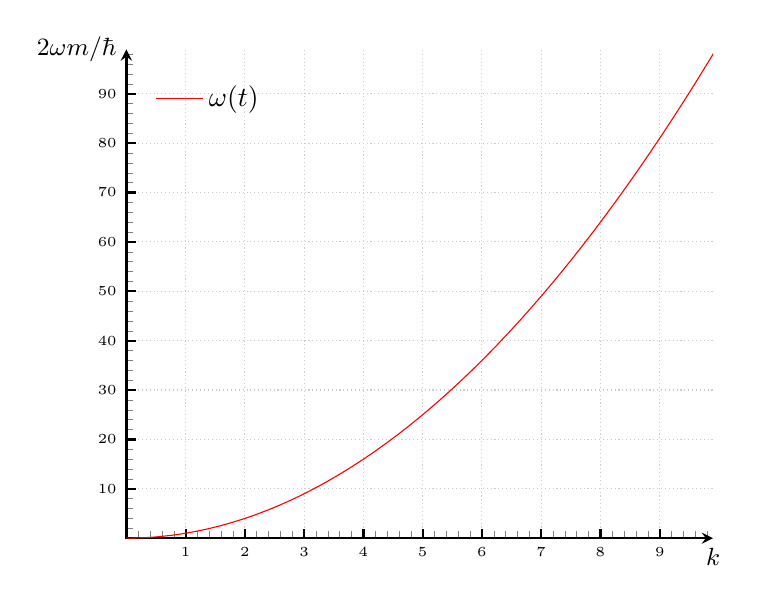
\begin{tikzpicture}
			\begin{axis}[
				every minor tick/.append style={minor tick length=0.085cm},
				every major tick/.append style={major tick length=0.12cm,thick,black},
				trig format plots=rad,
				width=257pt,
				height=222pt,
				axis lines=center,
				axis line style={thick},
				tick align=outside,
				xmin=-0,xmax=9.9,ymin=-0.2,ymax=99,
				ticklabel style = {font=\tiny},
				tick align=inside,
				xlabel style={font=\small,below},
				ylabel style={font=\small,left},
				xtick distance=1,
				minor tick num=4,
				ytick distance=10,
				xlabel=$k$,
				ylabel=$2\omega m/\hbar$,
				grid=major,
				grid style={thin,densely dotted,black!20},
				legend columns=3,
				legend style={fill=none, draw=none, at={(axis description cs:0.25,0.9)},anchor=east}],
				\addplot [domain=0:10,smooth, red] {x^2};
				\legend{$\omega(t)$}
			\end{axis}
		\end{tikzpicture}
	\tcbline
		\item \( b = k - k_0;\quad \alpha = \sqrt{\tfrac{a^2}{4} + \tfrac{\iu\hbar t}{2m}};\quad \beta = \iu x - \tfrac{\iu\hbar k_0 t}{m};\quad \phi = -\tfrac{k_0^2\hbar}{2m}t - \tfrac{1}{2}\arctan(\tfrac{2\hbar t}{ma^2}) \)
		\begin{flalign*}
			\psi(x, t) &= \tfrac{\sqrt{a}}{(2\pi)^{3/4}} \uint[-\infty,\infty]{\exp\bigg(-\tfrac{a^2}{4}(k - k_0)^2 \bigg)\exp\bigg(\iu(kx - \omega(k)t) \bigg)}{k} = &&\\
			&\hspace{-4pt}\stackrel{\text{u-sub}}{=} \tfrac{\sqrt{a}}{(2\pi)^{3/4}} \uint[-\infty,\infty]{\exp\bigg(-\tfrac{a^2}{4}b^2 \bigg)\exp\bigg(\iu(k(b + k_0) - \tfrac{\hbar (b + k_0)^2}{2m}t) \bigg)}{b} = &&\\
			&= \tfrac{\sqrt{a}}{(2\pi)^{3/4}} \exp\big(\iu k_0 x \big) \exp\bigg(-\iu t\tfrac{k_0^2 \hbar}{2m} \bigg) \uint[-\infty,\infty]{\exp\big( \beta b \big) \exp\big( -\alpha^2b^2 \big)}{b} = &&\\
			&= \tfrac{\sqrt{a}}{(2\pi)^{3/4}} \exp\big(\iu k_0 x \big) \exp\big( \iu\phi \big) \tfrac{\exp\bigg( \tfrac{\beta^2}{4\alpha^2} \bigg) \sqrt{\pi}}{\alpha} = &&\\
			&= \dl{\left( \tfrac{2a^2}{\pi} \right)^{1/4} \tfrac{\exp\big( \iu\phi \big)}{\left( a^4 + \tfrac{4\hbar^2 t^2}{m^2} \right)^{1/4}} \exp\big(\iu k_0 x \big) \exp\left( \tfrac{\left(x - \tfrac{\hbar k_0}{m}t \right)^2}{a^2 + \tfrac{2\iu \hbar t}{m}} \right)} &&
		\end{flalign*}
		\begin{flalign*}
			\abs{\psi(x, t)}^2 &= \sqrt{\tfrac{2a^2}{\pi\left( a^4 + \tfrac{4\hbar^2 t^2}{m^2} \right)}} \exp\big(2\iu k_0 x \big) \exp\big(2\iu\phi \big) \exp\left(\tfrac{\left(x - \tfrac{\hbar k_0}{m}t \right)^2}{a^2 + \tfrac{2\iu \hbar t}{m}} \right) = &&\\
			=& \dl{\sqrt{\frac{1}{2\sigma^2(t)}} \exp\left( -\tfrac{\left(x - \tfrac{\hbar k_0}{m}t \right)^2}{2\sigma^2(t)} \right)} &&
		\end{flalign*}
	\tcbline
		\item %
		\pgfmathdeclarefunction{gauss}{2}{%
			\pgfmathparse{1/(#2*sqrt(2*pi))*exp(-((x-#1)^2)/(2*#2^2))}%
		}
		\begin{tikzpicture}
			\begin{axis}[
				every minor tick/.append style={minor tick length=0.085cm},
				every major tick/.append style={major tick length=0.12cm,thick,black},
				trig format plots=rad,
				width=257pt,
				height=222pt,
				axis lines=center,
				axis line style={thick},
				tick align=outside,
				xmin=-5.5,xmax=5.5,ymin=-0,ymax=0.99,
				ticklabel style = {font=\tiny},
				tick align=inside,
				xlabel style={font=\small,below},
				ylabel style={font=\small,left},
				xtick distance=1,
				minor tick num=4,
				ytick distance=0.5,
				xlabel=$t$,
				ylabel=,
				grid=major,
				grid style={thin,densely dotted,black!20},
				legend style={fill=none, draw=none, at={(axis description cs:0.4,0.8)},anchor=east}],
				\addplot[smooth, mark=none, samples=50, color=magenta, thick] {gauss(-1,0.75)};
				\addplot[smooth, mark=none, samples=50, color=blue, thick] {gauss(0,0.5)};
				\addplot[smooth, mark=none, samples=50, color=red, thick] {gauss(2,1)};
				\legend{$\abs{\psi(t < 0)}^2$~~~,$\abs{\psi(t = 0)}^2$~~~,$\abs{\psi(t > 0)}^2$}
			\end{axis}
		\end{tikzpicture}
		\begin{flalign*}
			-\frac{1}{2} &= -\tfrac{\left(2\delta x(t) - \tfrac{\hbar k_0}{m}t \right)^2}{2\sigma^2(t)}\quad \Leftrightarrow\quad 2\delta x(t) = \sqrt{\sigma^2(t)} - \tfrac{\hbar k_0}{m}t &&\\
			\delta x(t) &= \dl{\tfrac{\sqrt{\sigma^2(t)} - \tfrac{\hbar k_0}{m}t}{2}} &&
		\end{flalign*}
	\end{enumerate}
\end{mybox}


\end{document}